\documentclass[aspectratio=169]{beamer}
\setbeamerfont{headline}{size=\footnotesize}

\mode<presentation>{
    \usetheme{Montpellier}
    \setbeamercovered{transparent}
    \usecolortheme{beaver}
}

\usepackage[english,brazil]{babel}
\usepackage[utf8]{inputenc}
\usepackage{fontawesome}
\usepackage{graphicx}
\usepackage{listings}
\usepackage{url}
\usepackage{colortbl}
\usepackage{caption}
\usepackage{ragged2e}
\usepackage{booktabs}
\usepackage{multirow}
\usepackage{array}
\usepackage{scalefnt}

% Colors
\definecolor{mineblue}{RGB}{0,90,180}
\definecolor{mineorange}{RGB}{230,115,0}
\definecolor{minegreen}{RGB}{34,139,34}
\definecolor{minered}{RGB}{180,20,40}
\definecolor{minegray}{RGB}{100,100,100}
\definecolor{codegreen}{rgb}{0,0.6,0}
\definecolor{codegray}{rgb}{0.5,0.5,0.5}
\definecolor{codepurple}{rgb}{0.58,0,0.82}
\definecolor{backcolour}{rgb}{0.95,0.95,0.92}

\usepackage{tikz}
\usetikzlibrary{arrows.meta,shapes.geometric,positioning,fit,backgrounds,calc,trees}
\usepackage{pgfplots}
\pgfplotsset{compat=1.18}

\newcommand{\reflexao}[1]{\begin{alertblock}{Reflexão}#1\end{alertblock}}
\newcommand{\key}[1]{\underline{#1}}

% Tikz styles
\tikzstyle{block} = [rectangle, draw, fill=blue!20, text width=5em, text centered, rounded corners, minimum height=4em]
\tikzstyle{line} = [draw, -latex']

% Author info
\title[Mineração de Dados]{Mineração de Dados: Conceitos e Aplicações}
\subtitle{Módulo 2: Pré-processamento de Dados}
\author[Elton Sarmanho]{Prof. Elton Sarmanho\inst{1}\\\footnotesize \href{mailto:eltonss@ufpa.br}{eltonss@ufpa.br}}
\institute[UFPA]{\inst{1} Faculdade de Sistemas de Informação - UFPA Campus Cametá}
\date{\today}

\begin{document}

%============================================================
% Slide 1: Título
%============================================================
\begin{frame}
    \titlepage
    \begin{center}
        \tiny \faGithub \ \href{https://github.com/eltonsarmanho}{github.com/eltonsarmanho} \quad
        \faLinkedinSquare \ \href{https://www.linkedin.com/in/elton-sarmanho-836553185/}{Elton Sarmanho}
    \end{center}
\end{frame}

%============================================================
% Slide 2: Roteiro
%============================================================
\begin{frame}{Roteiro da Aula}
    \tableofcontents
\end{frame}

%============================================================
\section{Qualidade de Dados}
%============================================================

\begin{frame}{Por que Pré-processar os Dados?}
    \footnotesize
    \begin{columns}[T]
        \column{0.42\textwidth}
        \begin{alertblock}{Regra 80-20}
            \textbf{80\%} do tempo de um projeto de ciência de dados é gasto em \textbf{pré-processamento}; apenas 20\% em modelagem.
        \end{alertblock}
        \vspace{0.3em}
        Dados do mundo real chegam:
        \begin{itemize}
            \item Incompletos (valores ausentes)
            \item Inconsistentes (duplicatas, erros)
            \item Desbalanceados (classes raras)
            \item Em escalas diferentes
        \end{itemize}

        \column{0.55\textwidth}
        \textbf{6 Dimensões de Qualidade de Dados:}
        \vspace{0.3em}

        \begin{columns}[T]
            \column{0.5\textwidth}
            \begin{block}{\small Acurácia}
                \tiny Dados refletem a realidade?
            \end{block}
            \begin{block}{\small Completude}
                \tiny Dados necessários presentes?
            \end{block}
            \begin{block}{\small Consistência}
                \tiny Dados coerentes entre si?
            \end{block}

            \column{0.5\textwidth}
            \begin{block}{\small Temporalidade}
                \tiny Dados estão atualizados?
            \end{block}
            \begin{block}{\small Validade}
                \tiny Dentro dos domínios esperados?
            \end{block}
            \begin{block}{\small Unicidade}
                \tiny Sem duplicatas indevidas?
            \end{block}
        \end{columns}
    \end{columns}
\end{frame}

%============================================================
\section{Tipos de Dados}
%============================================================

\begin{frame}{}
    \footnotesize
    \vspace{-0.2cm}

    \begin{center}
    \small
    \begin{tabular}{>{\bfseries\color{mineblue}}p{2.0cm} p{3.2cm} p{4.5cm}}
        \toprule
        \textbf{Escala} & \textbf{Característica} & \textbf{Exemplos} \\
        \midrule
        Nominal & Apenas categorias, sem ordem & Cor dos olhos, Estado civil, Tipo sanguíneo \\
        \midrule
        Ordinal & Categorias com ordem; intervalos desiguais & Satisfação (1--5), Grau de escolaridade \\
        \midrule
        Intervalar & Intervalos iguais; zero arbitrário & Temperatura (°C), Ano calendário \\
        \midrule
        Razão & Intervalos iguais; zero absoluto & Peso (kg), Altura (cm), Renda (R\$) \\
        \bottomrule
    \end{tabular}
    \end{center}

    \begin{columns}[T]
        \column{0.5\textwidth}
        \begin{exampleblock}{Estruturados vs.\ Não Estruturados}
            \small Dados tabulares (SQL) vs.\ texto, imagem, áudio, que requerem extração de features.
        \end{exampleblock}

        \column{0.5\textwidth}
        \begin{exampleblock}{Séries Temporais e Espaciais}
            \small Sequências ordenadas no tempo ou com componente geográfico, exigindo técnicas especiais.
        \end{exampleblock}
    \end{columns}
\end{frame}

%============================================================
\section{Dados Ausentes}
%============================================================

\begin{frame}{Mecanismos de Ausência: MCAR, MAR e MNAR}
    \begin{columns}[T]
        \column{0.33\textwidth}
        \begin{block}{\color{mineblue} MCAR}
            \textbf{Missing Completely At Random}\\[0.3em]
            \small A ausência \textbf{não depende} de nenhum dado.\\[0.3em]
            \textit{Ex.:} Sensor falha aleatoriamente a cada 1000 medições.\\[0.3em]
            \footnotesize \textbf{Tratamento:} Remoção de registros (sem viés), porém perde poder estatístico.
        \end{block}

        \column{0.33\textwidth}
        \begin{block}{\color{mineorange} MAR}
            \textbf{Missing At Random}\\[0.3em]
            \small Ausência depende de \textbf{outras variáveis observadas}.\\[0.3em]
            \textit{Ex.:} Pessoas com alta renda tendem a não informar renda (dependendo de escolaridade).\\[0.3em]
            \footnotesize \textbf{Tratamento:} Imputação múltipla (MICE).
        \end{block}

        \column{0.33\textwidth}
        \begin{block}{\color{minered} MNAR}
            \textbf{Missing Not At Random}\\[0.3em]
            \small Ausência depende do \textbf{próprio valor ausente}.\\[0.3em]
            \textit{Ex.:} Pacientes com pressão muito alta faltam às consultas.\\[0.3em]
            \footnotesize \textbf{Tratamento:} Modelagem explícita do mecanismo: qualquer imputação simples introduz viés.
        \end{block}
    \end{columns}
\end{frame}

\begin{frame}{Padrões de Ausência: Visualização}
    \begin{center}
    \scalebox{0.65}{%
    \begin{tikzpicture}[
      cell/.style={rectangle,minimum width=0.5cm,minimum height=0.5cm,
                   draw=minegray!50,inner sep=0pt}]

      \node[font=\small\bfseries,color=mineblue]   at (1.5, 3.0)  {MCAR};
      \node[font=\small\bfseries,color=mineorange] at (5.0, 3.0)  {MAR};
      \node[font=\small\bfseries,color=minered]    at (8.5, 3.0)  {MNAR};

      % Grade MCAR
      \foreach \c in {1,...,6}{
        \foreach \r in {1,...,5}{
          \node[cell,fill=mineblue!15] at ({(\c-0.5)*0.5},{(\r-0.5)*0.5}) {};
        }
      }
      \node[cell,fill=minered!60] at (0.25,1.75) {};
      \node[cell,fill=minered!60] at (1.25,2.25) {};
      \node[cell,fill=minered!60] at (2.75,0.25) {};
      \node[cell,fill=minered!60] at (2.25,1.75) {};
      \node[cell,fill=minered!60] at (0.75,0.75) {};
      \node[cell,fill=minered!60] at (1.75,1.25) {};
      \node[font=\tiny,align=center,text width=3.2cm] at (1.5,-0.4)
        {Ausências distribuídas\\aleatoriamente};

      % Grade MAR
      \foreach \c in {1,...,6}{
        \foreach \r in {1,...,5}{
          \node[cell,fill=mineorange!15] at ({(\c-0.5)*0.5+3.5},{(\r-0.5)*0.5}) {};
        }
      }
      \node[cell,fill=minered!60] at (5.75,1.25) {};
      \node[cell,fill=minered!60] at (6.25,1.25) {};
      \node[cell,fill=minered!60] at (5.75,1.75) {};
      \node[cell,fill=minered!60] at (6.25,1.75) {};
      \node[cell,fill=minered!60] at (5.75,2.25) {};
      \node[cell,fill=minered!60] at (6.25,2.25) {};
      \node[font=\tiny,align=center,text width=3.2cm] at (5.0,-0.4)
        {Ausências dependem de\\outras variáveis observadas};

      % Grade MNAR
      \foreach \c in {1,...,6}{
        \foreach \r in {1,...,5}{
          \node[cell,fill=minered!10] at ({(\c-0.5)*0.5+7.0},{(\r-0.5)*0.5}) {};
        }
      }
      \node[cell,fill=minered!60] at (9.75,1.25) {};
      \node[cell,fill=minered!60] at (9.75,1.75) {};
      \node[cell,fill=minered!60] at (9.75,2.25) {};
      \node[font=\tiny\itshape,anchor=west] at (10.1,0.25) {baixo};
      \node[font=\tiny\itshape,anchor=west] at (10.1,0.75) {m\'{e}dio};
      \node[font=\tiny\itshape,anchor=west] at (10.1,1.25) {alto};
      \node[font=\tiny\itshape,anchor=west] at (10.1,1.75) {muito alto};
      \node[font=\tiny\itshape,anchor=west] at (10.1,2.25) {m\'{a}ximo};
      \node[font=\tiny,align=center,text width=3.2cm] at (8.5,-0.4)
        {Ausências nos maiores\\valores (sistêmico)};

      % Legenda
      \node[cell,fill=minered!60]  at (3.6,-1.0) {};
      \node[font=\tiny,anchor=west] at (3.85,-1.0) {: valor ausente};
      \node[cell,fill=mineblue!15] at (6.1,-1.0) {};
      \node[font=\tiny,anchor=west] at (6.35,-1.0) {: valor presente};
    \end{tikzpicture}
    }
    \end{center}
\end{frame}

\begin{frame}{Técnicas de Imputação}
    \begin{center}
    \small
    \begin{tabular}{>{\bfseries\color{mineblue}}p{2.8cm} p{3.5cm} p{3.5cm} p{2.5cm}}
        \toprule
        \textbf{Técnica} & \textbf{Como funciona} & \textbf{Quando usar} & \textbf{Limitação} \\
        \midrule
        Média / Mediana & Substitui pelo valor central da coluna & MCAR, $<5\%$ ausentes & Reduz variância \\
        \midrule
        KNN Imputer & Média ponderada dos $k$ vizinhos mais próximos & Relações locais entre instâncias & Custo $O(n^2)$ \\
        \midrule
        MICE & Cada coluna modelada por regressão iterativa & MAR; dados com relações complexas & Custo computacional \\
        \bottomrule
    \end{tabular}
    \end{center}

    \vspace{0.5em}
    \begin{alertblock}{Diagnóstico Primeiro!}
        \small A escolha da estratégia \textbf{deve ser precedida} do diagnóstico do mecanismo. Remover registros com MAR/MNAR introduz viés sistemático.
    \end{alertblock}
\end{frame}

%============================================================
\section{Outliers}
%============================================================

\begin{frame}{O que é um Outlier? Critério IQR}
    \begin{columns}[T]
        \column{0.4\textwidth}
        \begin{block}{Definição}
            \small Observação que se desvia significativamente do padrão esperado. Pode ser \textbf{erro de medição} ou \textbf{evento genuíno} (fraude, evento raro).
        \end{block}
        \vspace{0.5em}
        \textbf{Critério de Tukey (IQR):}
        \[IQR = Q_3 - Q_1\]
        \footnotesize Outlier se $x < Q_1 - 1.5 \cdot IQR$\\
        ou $x > Q_3 + 1.5 \cdot IQR$

        \column{0.58\textwidth}
        \begin{center}
        \scalebox{0.65}{%
        \begin{tikzpicture}[xscale=0.9]
          \draw[thick,mineblue,fill=mineblue!20] (3.0,0.5) rectangle (6.5,1.5);
          \draw[thick,minered,line width=2pt] (5.0,0.5) -- (5.0,1.5);
          \draw[thick,mineblue] (3.0,1.0) -- (1.5,1.0);
          \draw[thick,mineblue] (6.5,1.0) -- (8.5,1.0);
          \draw[thick,mineblue] (1.5,0.7) -- (1.5,1.3);
          \draw[thick,mineblue] (8.5,0.7) -- (8.5,1.3);
          \fill[minered] (-0.5,1.0) circle(4pt);
          \fill[minered] (10.0,1.0) circle(4pt);
          \fill[minered] (10.8,1.0) circle(4pt);
          \node[font=\small,below] at (3.0,0.5) {$Q_1$};
          \node[font=\small,below] at (5.0,0.5) {$Q_2$ (Med.)};
          \node[font=\small,below] at (6.5,0.5) {$Q_3$};
          \node[font=\tiny,below] at (1.5,0.5) {$Q_1 - 1.5 \cdot IQR$};
          \node[font=\tiny,below] at (8.5,0.5) {$Q_3 + 1.5 \cdot IQR$};
          \node[font=\small,minered,below] at (-0.5,0.5) {Outlier};
          \node[font=\small,minered,below] at (10.4,0.5) {Outliers};
          \draw[<->,minegreen,thick] (3.0,2.0) -- (6.5,2.0) node[midway,above,font=\small] {$IQR = Q_3 - Q_1$};
        \end{tikzpicture}
        }
        \end{center}
    \end{columns}
\end{frame}

\begin{frame}{Métodos de Detecção de Outliers}
    \begin{columns}[T]
        \column{0.48\textwidth}
        \begin{block}{Métodos Univariados}
            \begin{itemize}
                \item \textbf{Z-Score:} $z_i = \frac{x_i - \mu}{\sigma}$\\
                \footnotesize Outlier se $|z_i| > 3$. Sensível a extremos.
                \vspace{0.3em}
                \item \textbf{IQR (Tukey):}\\
                \footnotesize Robusto; usa quartis. Não assume normalidade.
                \vspace{0.3em}
                \item \textbf{Z-Score Modificado (MAD):}\\
                \footnotesize Usa mediana, extremamente robusto.
            \end{itemize}
        \end{block}

        \column{0.48\textwidth}
        \begin{block}{Métodos Multivariados / ML}
            \begin{itemize}
                \item \textbf{Isolation Forest:}\\
                \footnotesize Isola anomalias em menos divisões de árvore. Eficiente em alta dimensão.
                \vspace{0.3em}
                \item \textbf{LOF (Local Outlier Factor):}\\
                \footnotesize Compara densidade local com vizinhos. Detecta outliers locais.
                \vspace{0.3em}
                \item \textbf{One-Class SVM:}\\
                \footnotesize Aprende fronteira de normalidade. Pontos fora = anomalia.
            \end{itemize}
        \end{block}
    \end{columns}
\end{frame}

\begin{frame}{Como Tratar Outliers?}
    \begin{center}
    \small
    \begin{tabular}{>{\bfseries\color{mineblue}}p{2.5cm} p{3.5cm} p{3.5cm} p{2.5cm}}
        \toprule
        \textbf{Estratégia} & \textbf{Descrição} & \textbf{Quando usar} & \textbf{Cuidado} \\
        \midrule
        Remoção & Excluir registros com outliers & Erros claros de coleta & Pode perder dados raros legítimos \\
        \midrule
        Winsorização & Substituir pelos limites IQR & Extremos improváveis mas não impossíveis & Distorce distribuição original \\
        \midrule
        Transformação & Log, raiz quadrada, Box-Cox & Distribuição com cauda longa & Dificulta interpretação \\
        \midrule
        Manter & Não tratar & Outliers genuínos (fraude, doença rara) & Treinamento pode ser prejudicado \\
        \bottomrule
    \end{tabular}
    \end{center}
\end{frame}

%============================================================
\section{Normalização e Escalonamento}
%============================================================

\begin{frame}{Métodos de Normalização e Escalonamento}
    \begin{columns}[T]
        \column{0.48\textwidth}
        \begin{exampleblock}{Min-Max Normalization}
            $x'_i = \dfrac{x_i - x_{min}}{x_{max} - x_{min}} \in [0,1]$\\[0.3em]
            \footnotesize Mapeia para $[0,1]$. Sensível a outliers.
        \end{exampleblock}
        \vspace{0.4em}
        \begin{exampleblock}{Z-Score Standardization}
            $x'_i = \dfrac{x_i - \mu}{\sigma}$\\[0.3em]
            \footnotesize Média 0, desvio 1. Mais usado como padrão.
        \end{exampleblock}

        \column{0.48\textwidth}
        \begin{exampleblock}{Robust Scaler}
            $x'_i = \dfrac{x_i - Q_2}{IQR}$\\[0.3em]
            \footnotesize Usa mediana e IQR. Robusto a outliers.
        \end{exampleblock}
        \vspace{0.4em}
        \begin{exampleblock}{Transformação Logarítmica}
            $x'_i = \log(1 + x_i)$\\[0.3em]
            \footnotesize Reduz assimetria em distribuições com cauda longa. O $+1$ evita $\log(0)$.
        \end{exampleblock}
    \end{columns}

    \vspace{0.4em}
    \begin{alertblock}{Por que escalonar?}
        \small KNN, K-Means, SVM, PCA e redes neurais são \textbf{sensíveis a escala}. Árvores de decisão e gradient boosting \textbf{não precisam} de escalonamento.
    \end{alertblock}
\end{frame}

\begin{frame}{Guia de Escolha do Método de Escalonamento}

    \begin{center}
    \footnotesize
    \begin{tabular}{>{\bfseries\color{mineblue}}p{2.5cm} p{4.0cm} p{4.5cm}}
        \toprule
        \textbf{Método} & \textbf{Use quando} & \textbf{Não use quando} \\
        \midrule
        Min-Max & Redes neurais; dados sem outliers; range fixo necessário & Dados com outliers significativos \\
        \midrule
        Z-Score & Regressão linear/logística; SVM; PCA & Distribuições muito assimétricas \\
        \midrule
        Robust & Dados com outliers que devem ser mantidos & Algoritmos que exigem $[0,1]$ \\
        \midrule
        Log & Features com distribuição log-normal; contagens; preços & Dados com zeros: use $\log(1+x)$ \\
        \bottomrule
    \end{tabular}
    \end{center}
\end{frame}

%============================================================
\section{Seleção de Atributos}
%============================================================

\begin{frame}{Métodos de Seleção de Atributos}
    \begin{columns}[T]
        \column{0.55\textwidth}
        \begin{center}
        \scalebox{0.5}{%
        \begin{tikzpicture}[
          tree/.style={rectangle,rounded corners,draw=mineblue,fill=mineblue!10,
                       minimum width=1.5cm,minimum height=0.7cm,font=\small,align=center},
          edge from parent/.style={draw,->,thick},
          level 1/.style={sibling distance=5.5cm, level distance=1.6cm},
          level 2/.style={sibling distance=1.9cm, level distance=1.5cm}]
        \node[tree,fill=mineblue!30] {Seleção de\\Atributos}
          child { node[tree,fill=mineorange!20] {Filtro}
            child { node[tree,font=\tiny,fill=mineorange!10] {Correlação\\de Pearson} }
            child { node[tree,font=\tiny,fill=mineorange!10] {Informação\\Mútua} }
            child { node[tree,font=\tiny,fill=mineorange!10] {Chi-quadrado} }
          }
          child { node[tree,fill=minegreen!20] {Wrapper}
            child { node[tree,font=\tiny,fill=minegreen!10] {RFE} }
            child { node[tree,font=\tiny,fill=minegreen!10] {SFS / SBS} }
          }
          child { node[tree,fill=purple!20] {Embutido}
            child { node[tree,font=\tiny,fill=purple!10] {LASSO} }
            child { node[tree,font=\tiny,fill=purple!10] {Importância\\em Árvores} }
          };
        \end{tikzpicture}
        }
        \end{center}

        \column{0.42\textwidth}
        \begin{block}{\small Filtro}
            \footnotesize Avalia cada feature independentemente. Rápido, mas não considera interações entre features.
        \end{block}
        \vspace{0.3em}
        \begin{block}{\small Wrapper}
            \footnotesize Usa um algoritmo para avaliar subconjuntos. Mais preciso, mas computacionalmente caro.
        \end{block}
        \vspace{0.3em}
        \begin{block}{\small Embutido}
            \footnotesize Seleção durante o treinamento. LASSO zera coeficientes de features irrelevantes automaticamente.
        \end{block}
    \end{columns}
\end{frame}

%============================================================
\section{Balanceamento de Classes}
%============================================================

\begin{frame}{O Problema do Desbalanceamento de Classes}
    \begin{columns}[T]
        \column{0.5\textwidth}
        \begin{alertblock}{Exemplo: Detecção de Fraude}
            \small Dataset com \textbf{0.1\% de fraudes}: um modelo que sempre prevê ``não é fraude'' tem \textbf{99.9\% de acurácia} mas é completamente inútil!
        \end{alertblock}

        \vspace{0.5em}
        \textbf{Métricas corretas para dados desbalanceados:}
        \begin{itemize}
            \item Precision e Recall
            \item F1-Score
            \item AUC-ROC
        \end{itemize}

        \column{0.48\textwidth}
        \begin{block}{SMOTE: Como Funciona}
            \small Gera exemplos \textbf{sintéticos} da classe minoritária interpolando entre instâncias existentes:
            \[x_{new} = x_i + \lambda \cdot (x_{nn} - x_i)\]
            \footnotesize onde $x_{nn}$ é um vizinho aleatório e $\lambda \sim \mathcal{U}[0,1]$.\\[0.3em]
            Não copia instâncias existentes: \textbf{cria novas} no espaço de features.
        \end{block}
    \end{columns}
\end{frame}

\begin{frame}{Oversampling vs.\ Undersampling}
    \begin{center}
    \small
    \begin{tabular}{>{\bfseries\color{mineblue}}p{2.8cm} p{3.0cm} p{3.0cm} p{2.8cm}}
        \toprule
        \textbf{Estratégia} & \textbf{Vantagens} & \textbf{Desvantagens} & \textbf{Quando Usar} \\
        \midrule
        SMOTE & Aumenta diversidade; não perde dados & Pode gerar regiões irreais & Dataset pequeno a médio \\
        \midrule
        ADASYN & Foca nas regiões difíceis & Amplifica ruído & Fronteira de decisão complexa \\
        \midrule
        Random Under & Simples e rápido & Perde informação da classe majoritária & Dataset grande; custo computacional alto \\
        \midrule
        Tomek Links & Limpa a fronteira de decisão & Efeito modesto isoladamente & Pré-processamento complementar \\
        \bottomrule
    \end{tabular}
    \end{center}

    \vspace{0.4em}
    \begin{exampleblock}{Dica prática}
        \small Combine SMOTE + Tomek Links (SMOTETomek) para gerar sintéticos \textbf{e} limpar a fronteira ao mesmo tempo.
    \end{exampleblock}
    \end{frame}
\subsection{PCA}

\begin{frame}
\frametitle{Redução de Dimensionalidade}
\begin{itemize}
    \item Outra tarefa comum é a redução de dimensionalidade.
    \item O objetivo é mapear os dados de um espaço de alta dimensão \( \mathbb{R}^d \) para um espaço de menor dimensão \( \mathbb{R}^k \), onde \( k < d \).
    \item Um método popular é a \textbf{Análise de Componentes Principais} (PCA), que busca encontrar as direções de máxima variância nos dados.
    \item Matematicamente, o PCA resolve o problema de autovalores:
    \[
    \Sigma v = \lambda v,
    \]
    onde \( \Sigma \) é a matriz de covariância dos dados e \( v \) são os autovetores.
\end{itemize}
\end{frame}



\begin{frame}
\frametitle{Ilustração do PCA}
    \begin{figure}
        \centering
        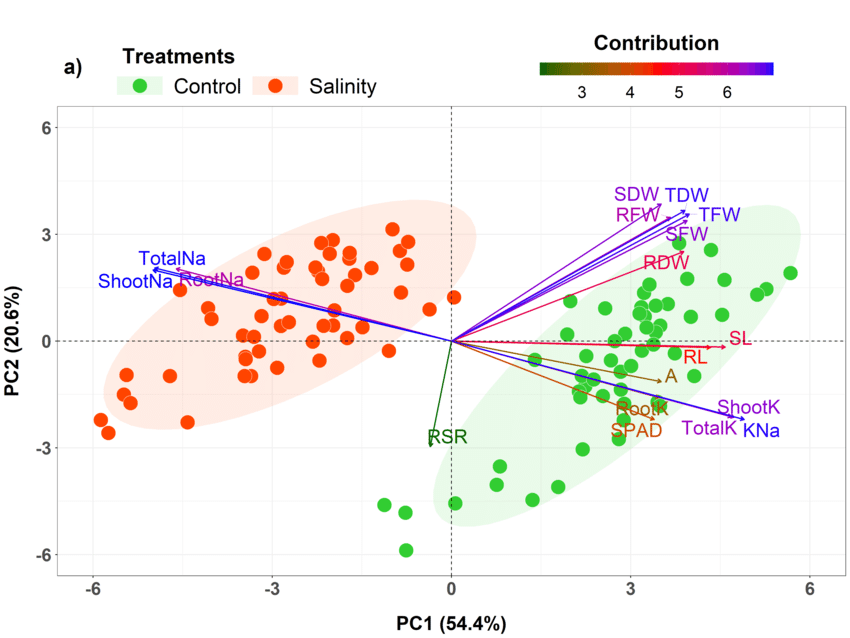
\includegraphics[scale=1.1]{figs/pca2.png}
    \end{figure}

\end{frame}


% ============================================================
% Slide: PCA — Intuição Geométrica
% ============================================================
\begin{frame}{Intuição Geométrica}
    \begin{center}
    \begin{tikzpicture}[scale=1.0]

        % Eixos originais (cinza, tracejado)
        \draw[->,minegray,dashed,thick] (-3.2,0) -- (3.4,0)
            node[right,font=\scriptsize\color{minegray}]{$x_1$};
        \draw[->,minegray,dashed,thick] (0,-2.0) -- (0,2.4)
            node[above,font=\scriptsize\color{minegray}]{$x_2$};

        % Nuvem de pontos (elipse inclinada ~35 graus)
        \foreach \px/\py in {
            -2.4/-1.1, -2.0/-0.9, -1.8/-0.6, -1.5/-0.5,
            -1.2/-0.3, -1.0/0.1,  -0.7/0.2,  -0.4/0.4,
             0.0/0.6,   0.3/0.5,   0.6/0.9,   1.0/1.0,
             1.3/1.3,   1.6/1.1,   1.9/1.5,  -1.6/-0.9,
            -0.9/-0.1,  0.5/0.7,   1.2/0.8,  -0.3/0.0}{
            \fill[mineblue!70] (\px,\py) circle (2.2pt);
        }

        % PC1 — direção de máxima variância (ângulo ~33°)
        \draw[->,very thick,minered]
            (-2.5,-1.2) -- (2.5,1.6)
            node[right,font=\scriptsize\bfseries\color{minered}]{$\mathbf{PC_1}$ (máx.\ variância)};

        % PC2 — ortogonal a PC1
        \draw[->,very thick,minegreen]
            (0.8,-1.6) -- (-0.8,1.3)
            node[above,font=\scriptsize\bfseries\color{minegreen}]{$\mathbf{PC_2}$};

        % Projeção de um ponto sobre PC1
        \fill[mineorange] (0.6,0.9) circle (3pt)
            node[above right,font=\tiny\color{mineorange}]{$\mathbf{p}$};
        % pé da projeção sobre PC1 (aprox.)
        \fill[minered!60] (0.95,0.6) circle (2.5pt)
            node[below right,font=\tiny\color{minered}]{$\hat{\mathbf{p}}$};
        \draw[mineorange,thick,dashed] (0.6,0.9) -- (0.95,0.6);

        % Legenda
        \node[font=\tiny,align=left] at (3.3,-1.5)
            {\textcolor{minered}{$\bullet$ PC$_1$: proj.\ máx.}\\
             \textcolor{minegreen}{$\bullet$ PC$_2$: ortog.}\\
             \textcolor{mineorange}{$\bullet$ $\hat p$: projeção de $p$}};

    \end{tikzpicture}
    \end{center}
    \vspace{-0.2cm}
    \begin{alertblock}{}
        \footnotesize O PCA rotaciona os eixos para que \textbf{PC\textsubscript{1}} capture a maior variância possível. Cada PC seguinte é ortogonal e captura o restante.
    \end{alertblock}
\end{frame}


% ============================================================
% Slide: PCA — Passo a Passo
% ============================================================
\begin{frame}{Algoritmo Passo a Passo}
    \begin{center}
    \begin{tikzpicture}[
        lbl/.style={font=\tiny,align=center,text width=3.2cm},
        scale=0.9]

        \node[rectangle,rounded corners,draw=mineblue,fill=mineblue!15,
              minimum width=2.6cm,minimum height=1.1cm,align=center,font=\scriptsize\bfseries]
              (s1) at (0,0)    {1.\\ Centralizar\\os dados};
        \node[rectangle,rounded corners,draw=mineorange,fill=mineorange!15,
              minimum width=2.6cm,minimum height=1.1cm,align=center,font=\scriptsize\bfseries]
              (s2) at (3.2,0)  {2.\\ Calcular\\covari\^{a}ncia};
        \node[rectangle,rounded corners,draw=minegreen,fill=minegreen!15,
              minimum width=2.6cm,minimum height=1.1cm,align=center,font=\scriptsize\bfseries]
              (s3) at (6.4,0)  {3.\\ Autovalores\\e Autovetores};
        \node[rectangle,rounded corners,draw=minered,fill=minered!15,
              minimum width=2.6cm,minimum height=1.1cm,align=center,font=\scriptsize\bfseries]
              (s4) at (9.6,0)  {4.\\ Selecionar\\$k$ PCs};
        \node[rectangle,rounded corners,draw=purple,fill=purple!15,
              minimum width=2.6cm,minimum height=1.1cm,align=center,font=\scriptsize\bfseries]
              (s5) at (12.8,0) {5.\\ Projetar\\os dados};

        \draw[->,thick,minegray] (s1.east)--(s2.west);
        \draw[->,thick,minegray] (s2.east)--(s3.west);
        \draw[->,thick,minegray] (s3.east)--(s4.west);
        \draw[->,thick,minegray] (s4.east)--(s5.west);

        \node[lbl] at (0,-1.6)    {Subtrair a\\média de cada\\atributo: $x \leftarrow x - \bar{x}$};
        \node[lbl] at (3.2,-1.6)  {Matriz $\Sigma$\\de covariância\\dos dados centrados};
        \node[lbl] at (6.4,-1.6)  {Resolver $\Sigma v = \lambda v$\\Autovetores = direções\\Autovalores = variâncias};
        \node[lbl] at (9.6,-1.6)  {Manter os $k$\\maiores autovalores\\(Scree Plot)};
        \node[lbl] at (12.8,-1.6) {$Z = X \cdot V_k$\\onde $V_k$ são os\\$k$ autovetores};

    \end{tikzpicture}
    \end{center}
    \vspace{0.1cm}
    \begin{alertblock}{}
        \footnotesize A centralização (passo 1) é \textbf{obrigatória}: sem ela, o PCA captura médias em vez de variâncias. A normalização também é recomendada quando os atributos têm escalas muito diferentes.
    \end{alertblock}
\end{frame}

% ============================================================
% Slide: PCA — Variância Explicada (Scree Plot)
% ============================================================
\begin{frame}{Variância Explicada: Scree Plot}
    \begin{center}
    \begin{tikzpicture}
    \begin{axis}[
        width=9cm, height=5.5cm,
        ybar,
        bar width=0.55cm,
        xlabel={Componente Principal},
        ylabel={Variância Explicada (\%)},
        xtick={1,2,3,4,5,6},
        xticklabels={PC$_1$,PC$_2$,PC$_3$,PC$_4$,PC$_5$,PC$_6$},
        ymin=0, ymax=55,
        ymajorgrids=true,
        grid style={dashed,minegray!30},
        axis lines=left,
        tick style={draw=none},
        label style={font=\small},
        tick label style={font=\small},
        nodes near coords,
        nodes near coords style={font=\tiny\bfseries},
        every axis plot/.append style={fill=mineblue!60,draw=mineblue},
    ]
        \addplot coordinates {(1,45) (2,25) (3,14) (4,9) (5,5) (6,2)};

        % Linha de variância acumulada 80%
        \draw[minered,very thick,dashed]
            (axis cs:0.4,35.5) -- (axis cs:6.6,35.5)
            node[right,font=\tiny\color{minered}]{};
    \end{axis}

    % Anotações fora do axis
    \node[font=\tiny\bfseries\color{minered},align=left] at (9.8,3.2)
        {$\sum$ PC$_1$+PC$_2$\\$= 70\%$};
    \node[font=\tiny\bfseries\color{minegreen},align=left] at (9.8,1.8)
        {$\sum$ PC$_1$+PC$_2$+PC$_3$\\$= 84\%$ \faCheck};

    \end{tikzpicture}
    \end{center}
    \vspace{-0.6cm}
    \begin{block}{Como escolher $k$?}
        \footnotesize Regra prática: selecionar o menor $k$ tal que a \textbf{variância acumulada} $\geq 80\text{--}95\%$. No exemplo acima, \textbf{$k=3$} captura 84\% da variância total com metade dos atributos originais.
    \end{block}
\end{frame}

%============================================================
% Referências
%============================================================
\section{Referências Bibliográficas}
\begin{frame}{Referências Bibliográficas}
    \begin{thebibliography}{99}
        \footnotesize
        \bibitem{garcia2015}
        GARCÍA, S. et al. \textit{Data Preprocessing in Data Mining}. Springer, 2015.
        \bibitem{chawla2002}
        CHAWLA, N. V. et al. SMOTE: Synthetic Minority Over-sampling Technique. \textit{JAIR}, v. 16, p. 321--357, 2002.
        \bibitem{vanbuuren2018}
        VAN BUUREN, S. \textit{Flexible Imputation of Missing Data}. 2. ed. CRC Press, 2018.
        \bibitem{liu2008}
        LIU, F. T. et al. Isolation Forest. \textit{ICDM}, 2008.
        \bibitem{tukey1977}
        TUKEY, J. W. \textit{Exploratory Data Analysis}. Addison-Wesley, 1977.
        \bibitem{tibshirani1996}
        TIBSHIRANI, R. Regression Shrinkage and Selection via the Lasso. \textit{JRSS-B}, v. 58, n. 1, 1996.
    \end{thebibliography}
\end{frame}

\begin{frame}[c]
    \begin{center}
        \Large \textbf{Consulte o Material Didático}\\[1em]
        \normalsize \textcolor{mineblue}{\textbf{Módulo 2: Pré-processamento de Dados}}\\[0.5em]
        \small Para aprofundamento nos conceitos, exemplos em Python,\\
        exercícios resolvidos e referências completas.\\[1.5em]
        \large \faGithub \ \href{https://github.com/eltonsarmanho}{github.com/eltonsarmanho}\\[0.5em]
        \href{mailto:eltonss@ufpa.br}{eltonss@ufpa.br}
    \end{center}
\end{frame}

\end{document}
